% Intended LaTeX compiler: xelatex
\documentclass[a4paper, 12pt]{article}
\usepackage{graphicx}
\usepackage{longtable}
\usepackage{wrapfig}
\usepackage{rotating}
\usepackage[normalem]{ulem}
\usepackage{amsmath}
\usepackage{amssymb}
\usepackage{capt-of}
\usepackage{hyperref}
\usepackage[danish]{babel}
\usepackage{mathtools}
\usepackage[margin=2.0cm]{geometry}
\hypersetup{colorlinks, linkcolor=black, urlcolor=blue}
\setlength{\parindent}{0em}
\parskip 1.5ex
\author{Jacob Debel}
\date{Fysik C \& B}
\title{Lys og bølger\\\medskip
\large Rekonstruktion - Brydning}
\hypersetup{
 pdfauthor={Jacob Debel},
 pdftitle={Lys og bølger},
 pdfkeywords={},
 pdfsubject={},
 pdfcreator={Emacs 29.4 (Org mode 9.6.15)}, 
 pdflang={Danish}}
\begin{document}

\maketitle


\section*{\(c\)}
\label{sec:orgaaebbf1}
\begin{minipage}{0.3\linewidth}
\begin{itemize}
\item Hvad er fagord,  værdi og enhed for \(c\)?
\end{itemize}
\end{minipage}
\vline
\begin{minipage}{0.68\linewidth}
Lyset bevæger sig igennem luft, som kan betragtes som vakuum.
\begin{center}
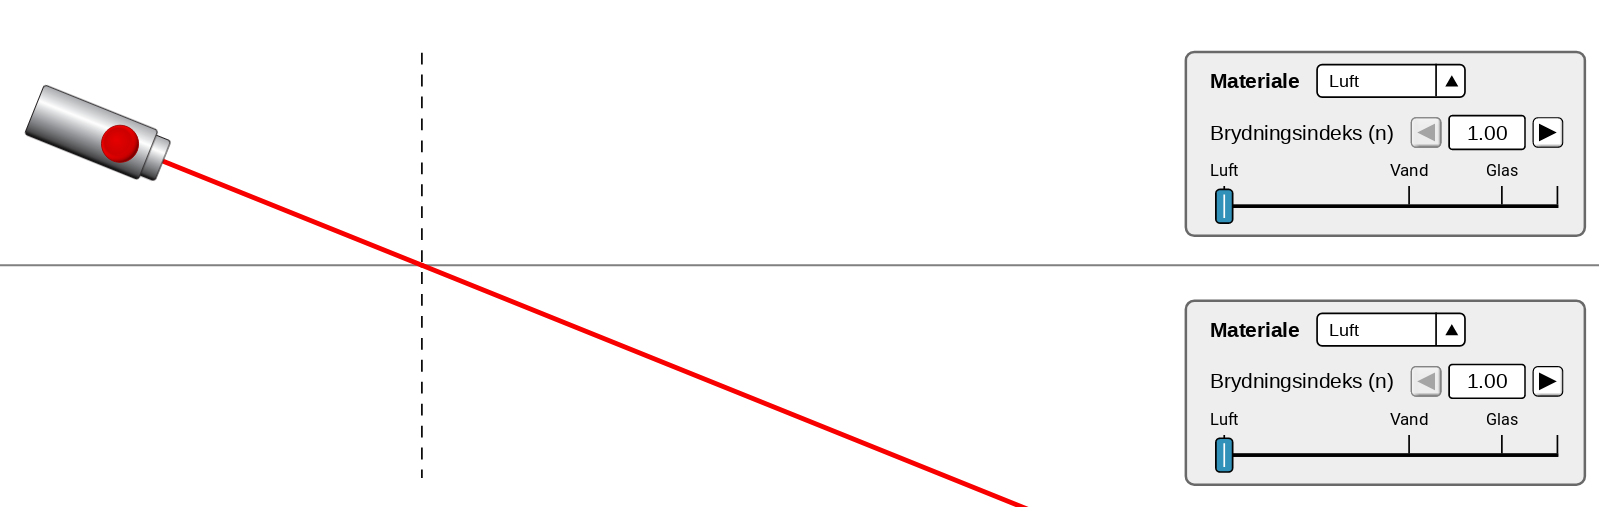
\includegraphics[width=.9\linewidth]{./img/laser_luft_luft.png}
\end{center}
\end{minipage}

\vfill
\section*{\(n\) og \(v\)}
\label{sec:org46cef88}
\begin{minipage}{0.3\linewidth}
\begin{itemize}
\item Hvad er fagordene og enhederne for \(n\) og \(v\)?
\end{itemize}
\end{minipage}
\vline
\begin{minipage}{0.68\linewidth}
\begin{center}
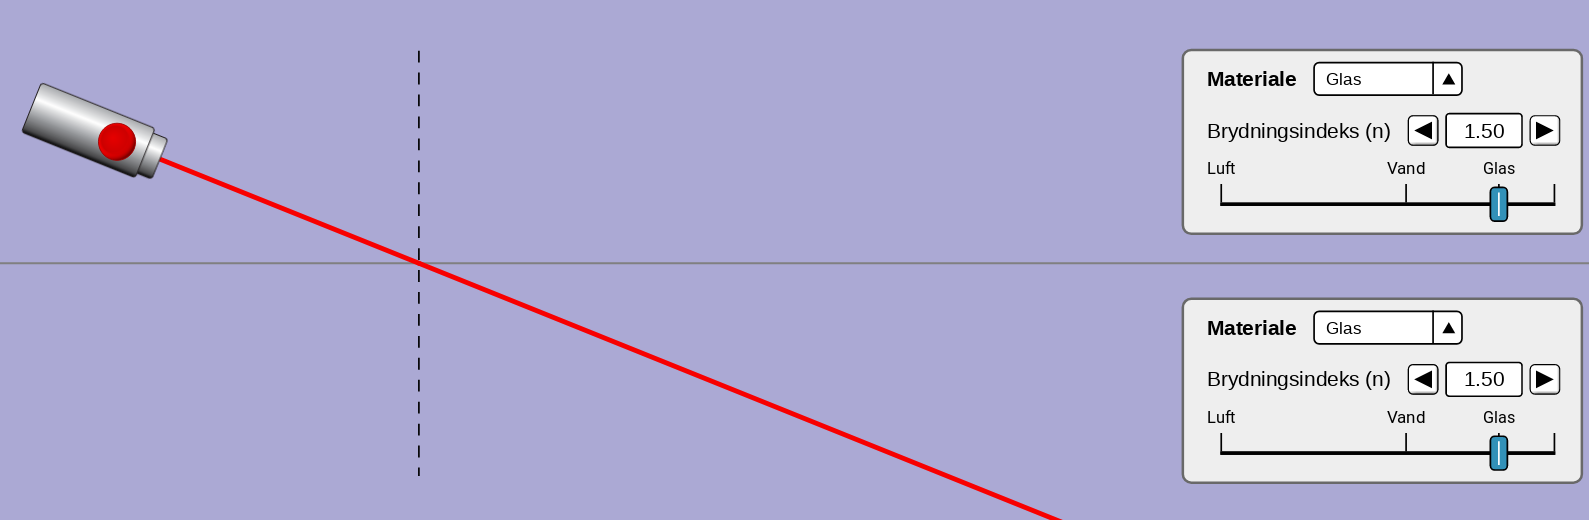
\includegraphics[width=.9\linewidth]{./img/laser_glas_glas.png}
\end{center}
\end{minipage}

\vfill
\newpage


\section*{\(v_1\) og \(v_2\)}
\label{sec:org915d1f4}

\begin{minipage}{0.3\linewidth}
\begin{itemize}
\item Hvad er \(v_1\) og \(v_2\)?
\item Hvilken er størst af de to?
\item Hvad sker der med lysets hastighed, når det passerer fra materiale 1 til materiale 2?
\end{itemize}
\end{minipage}
\vline
\begin{minipage}{0.68\linewidth}
Lyset bevæger sig fra et materiale, luft, til et andet materiale, glas.
\begin{center}
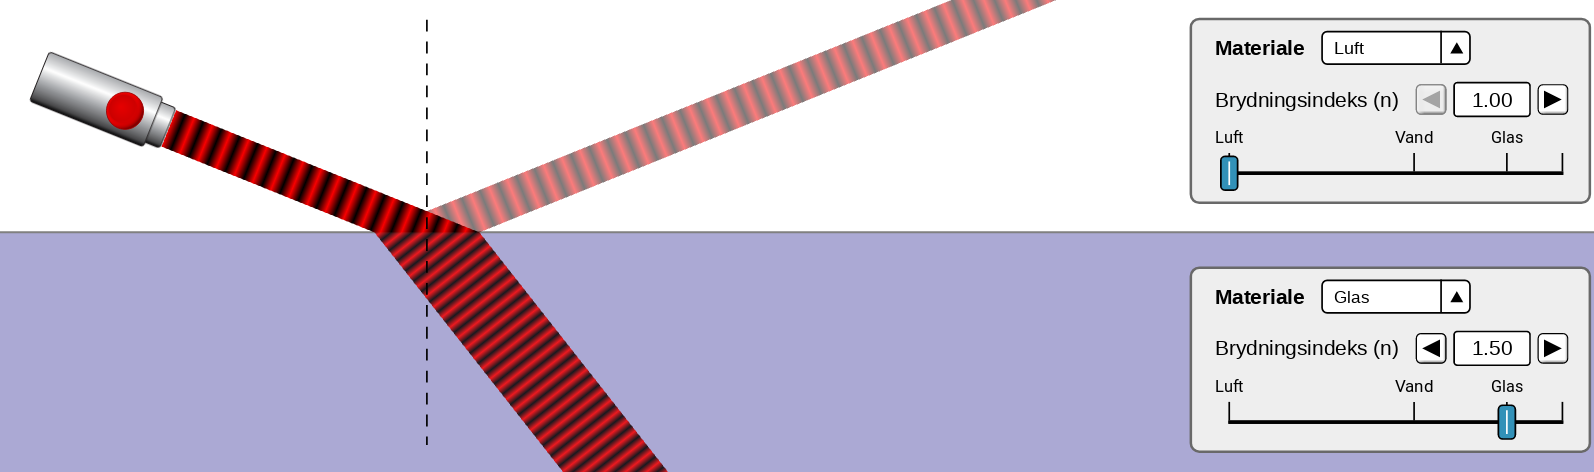
\includegraphics[width=.9\linewidth]{./img/laser_luft_glas.png}
\end{center}  
\end{minipage}


\vfill

\section*{\(i\) og \(b\)}
\label{sec:org860f0ce}

\begin{minipage}{0.3\linewidth}
\begin{itemize}
\item Hvor er \(i\) og \(b\) på figuren?
\item Hvad er fagordene for \(i\) og \(b\)?
\item Hvor måles de fra?
\end{itemize}
\end{minipage}
\vline
\begin{minipage}{0.68\linewidth}
\begin{center}
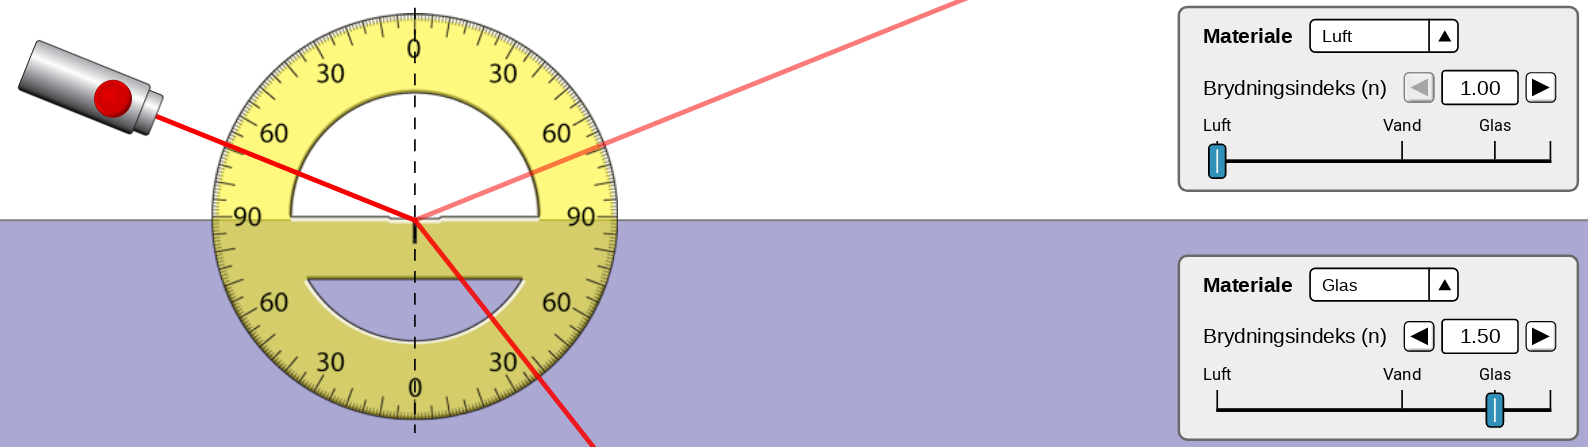
\includegraphics[width=.9\linewidth]{./img/laser_luft_glas_vinkel.png}
\end{center}
\end{minipage}

\vfill
\newpage

\section*{Lysets brydning}
\label{sec:orgde9ff30}
\begin{minipage}{0.3\linewidth}
\begin{itemize}
\item Hvordan forklarer man, at lys brydes (skrifter regning), når det går fra et materiale til et andet?
\end{itemize}
\end{minipage}
\vline
\begin{minipage}{0.68\linewidth}
\begin{center}
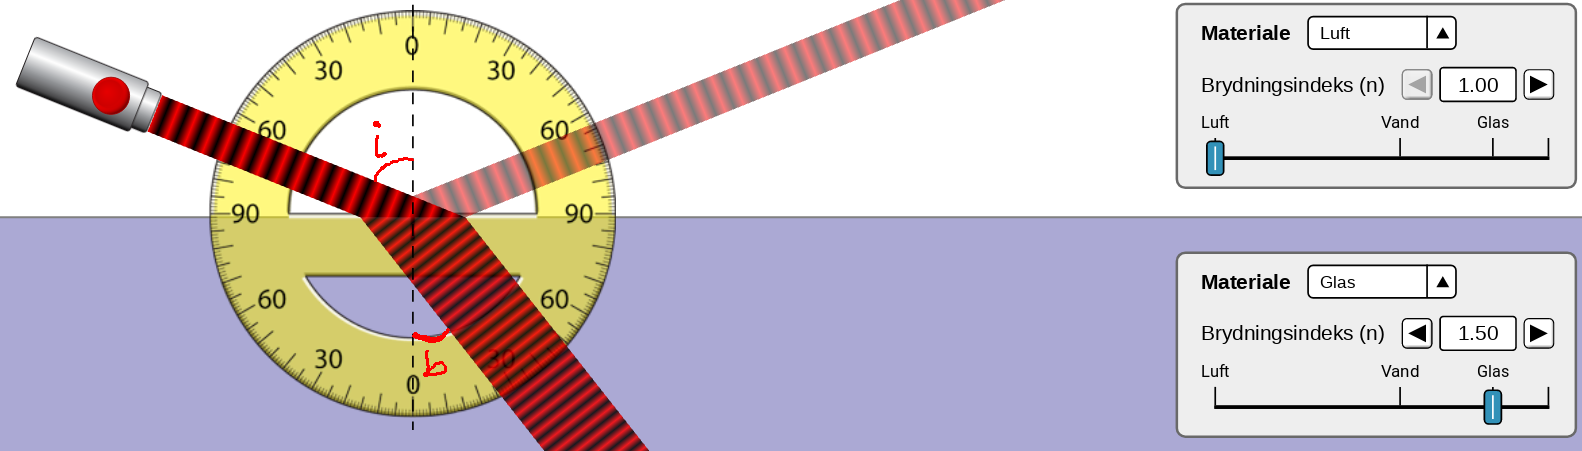
\includegraphics[width=.9\linewidth]{./img/laser_luft_glas_i_og_b.png}
\end{center}
\end{minipage}

\vfill



\section*{Totalrefleksion}
\label{sec:org9574cd7}

\begin{minipage}{0.3\linewidth}
\begin{itemize}
\item Hvordan forklarer man, hvornår totalrefleksion kan opstå?
\item Hvor er grænsevinklen for totalrefleksion på figuren?
\end{itemize}
\end{minipage}
\vline
\begin{minipage}{0.68\linewidth}
\begin{center}
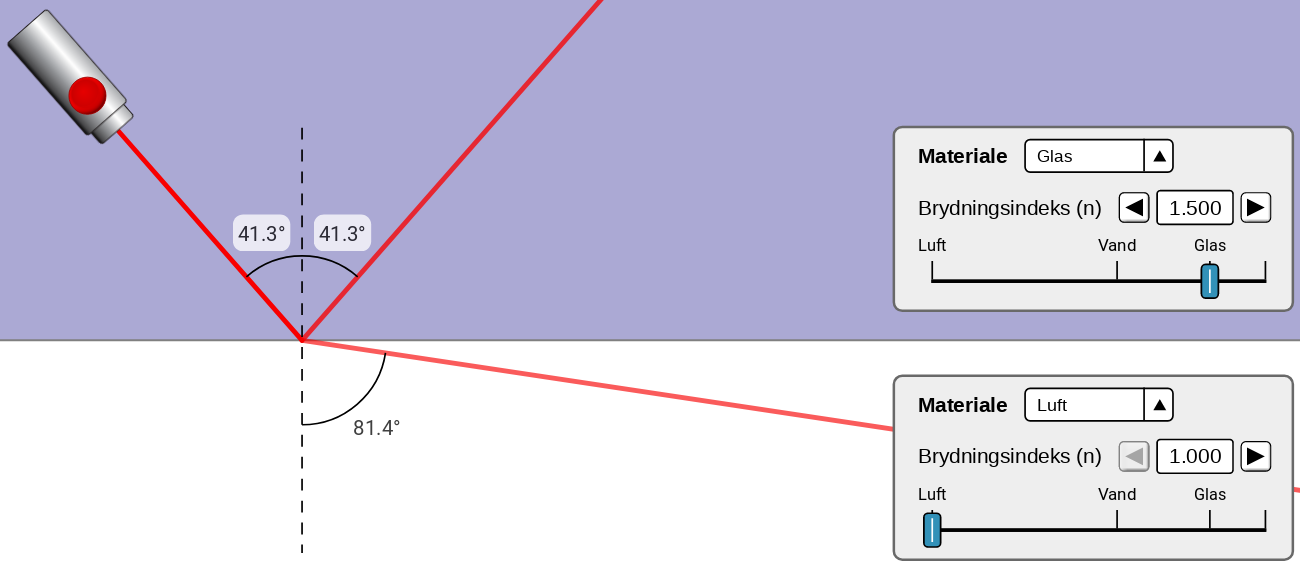
\includegraphics[width=.9\linewidth]{./img/totalrefleksion_1.png}
\end{center}
\begin{center}
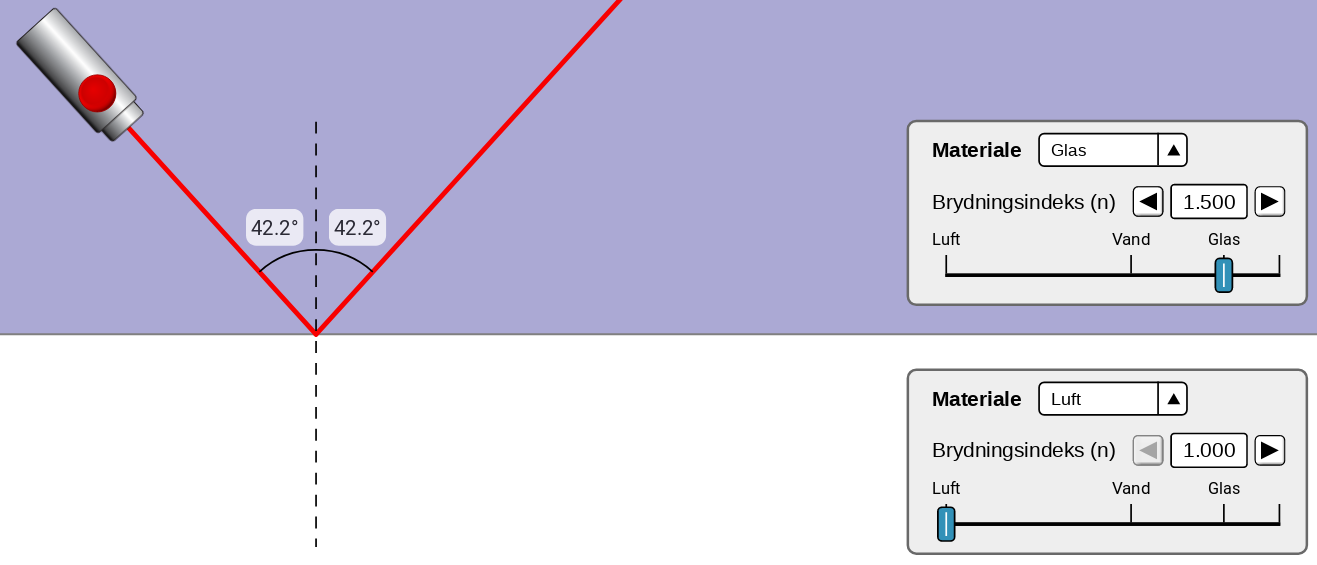
\includegraphics[width=.9\linewidth]{./img/totalrefleksion_2.png}
\end{center}
\end{minipage}
\end{document}
